The goal of this project is to develop a system that has atonomously learned from the handovers performed by humans to output an object's settings for how to be handed over, given an image of it. Another of our requirements is that the learning has been abstracted enough that this system is also accurately applicable on new objects that are not present in the training set. One way to go about with this would be by learning the handover settings for an object and then training for object classification. In other words, record all the handover features for each individual object, create a mean from them, and train a machine to recognize the object based on images as to output its settings. Such a machine would for \(n\) number of objects learn to output \(n\) different classes. This can potentially become an increasingly difficult task as the dataset of objects grows. At the same time as the requirements on the size for the dataset grows to be able to learn to properly recognize the objects. Such a system would believe that each object has its settings. If we instead hypothesize that some objects are handed over in similar fashion we can try a different approach:  letting the system, through unsupervised learning, find relationships between the observations of handovers and through this classify the individual objects into classes of handovers. This simplifies our problem as the number of outputs shrinks. We no longer pressure the system into properly recognizing invidual objects, but instead similarities between those that share the same features, which also lowers the requirements on data collection.

The first part of this work will be to observe and record a number of handovers between humans for a defined set of objects which the system will the try to categorise into different classes. In a second part each object will then be assigned a class that we train a machine to return when given an image. Seeing how we do not have any labels for the handovers, but still want to train a model that outputs some defined class for how the object should be handed over, we will be using a semi-supervised approach in this project: by first applying an unsupervised learning algorithm to categorise and create classes of handovers that are later used as output through self-supervised learning.

\section{Tools and material}

\subsection*{Hardware}

During the project the following material were used:

\begin{description}
	\item[Kinect for Windows v2] Motion sensing device developed by Microsoft used for recording and taking pictures with support for color, depth and infrared data.

	\item[GeForce GTX 980 Ti] Nvidia brand GPU for better performance during training of for example deep neural networks that require a lot of data and processing power.

	\item[\textcite{AprilTags}] In order to extract data from the recorded frames about the objects we need to detect the objects themselves. Object detection is a very difficult part of computer vision and there are many different methods, where some are more robust than others, to do so. To help with this part to make data extraction easier and more precise we will be taking help of AprilTags. AprilTags can be compared to QR-codes that are printed out on small papers and fastened onto the objects. With the help of their software library we can easily track the objects in the recorded material by getting the position of the four corners of the tag, and its center, which enables us to estimate such things as pose of the object.

	\item[Fifteen different objects to be handed over] Chosen randomly around the house, all of which can be handed over using only one hand with ease. The set objects include: a knife, a screwdriver, a can, a box, a pair of cutters, a tube, a pitcher, a glass, a bottle, a brush, a cup, a hammer, a pen, a scalpel and a pair of scissors.

\end{description}

\begin{figure}
	\centering
	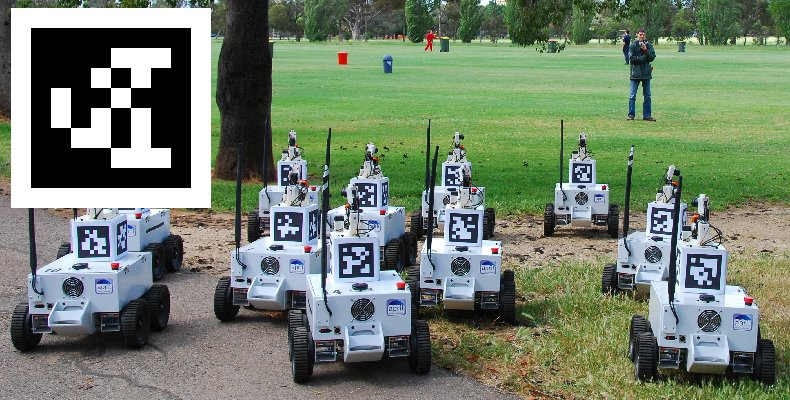
\includegraphics[width=\textwidth]{img/methods/apriltagrobots_overlay.jpg}
	\caption{Example of AprilTags in use on robots.}
\end{figure}

\subsection*{Software}

The applications will be written mostly in C++ or Python depending on availability of libraries. To help implement our system we will have the following programs and programming libraries at our disposal:

\begin{description}
	\item[\textcite{GIMP}] Image editing program that will be used for manual preprocessing of some images.

	\item[\textcite{libfreenect2}] Open source library written in C++ for communicating with the Kinect v2 camera.

	\item[\textcite{OpenCV}] Open source library for computer vision with bindings for C++ and Python, as well as other languages.

	\item[AprilTags programming library] C++ library written by the creators of AprilTag to help extract data from captured images such as the four corners of the tag and center of the tag.

	\item[\textcite{scikitlearn}] Python machine-learning library. Contains several useful tools for implementing and training models, as well as data processing.

	\item[\textcite{Tensorflow}] Open source Python library for creating and training neural networks with GPU support for more efficient processing time.

\end{description}


\section{Categorisation of handovers}

\subsection{Collection of data: recording of handovers}

For this purpose a number of voluteers were asked to be recorded while handing over a set of objects between each other. Even though Kinect v2 supports depth images, only two-dimensional color data will be used in this part. A total of 11 people who already knew each other from before volunteered (including myself) for this task. Pairs of volunteers were permuted as to try and make each person while being the giver adapt to different receivers. Instructions for handing over the objects were given prior to recordings as to make sure participants gave the object in a manner that the person receiving the object can use it straight away after grasping it. For example the hammer should be handed over with its handle first in a manner that the next person can start hammering directly without requiring a switch of grip after receiving it. Or a cup is to be handed handle-first so the person can start drinking right away. A bottle is easier to pour from if you hold it below its center of gravity therefore this area should be free for the receiving person while handing it over. For reasons that we will see later participants were instructed to use a grasp that covers the object, they could not for example hand something over flat in their palm. This is because of how the grasp region is identified and its limitations. The general regions of where to grasp by the giver and what part to present to the person receiving were chosen by myself with in mind for optimization for the receiver when given the object. For objects that might contain liquids the participants were asked to imagine that these objects were filled to the top while handing them over between each other.

\subsection{Extracting features}

% TODO write more about image moments
% TODO write about homography

\subsubsection{Orientation of the object}

The first set of features that we will extract from the recorded material will be around the orientation of the object when being handed over, i.e. the transformation from its ground truth to the observed position. Before any work is done with the recorded material, for each object we manually create a reference image representing its ground truth position. The orientation of the ground truth was chosen to be the object's orientation while in comon resting position (e.g for a bottle, standing up). For those objects that are layed down, their orientation was chosen to be with their head upwards. From these images we also generate binary masks that will be used to mask out the object after detection. Figure \ref{fig:objects_montage} shows the reference images created and figure \ref{fig:masks_montage} shows their binary masks. These images were created using the image manipulation software GIMP.

\begin{figure}
	\centering
	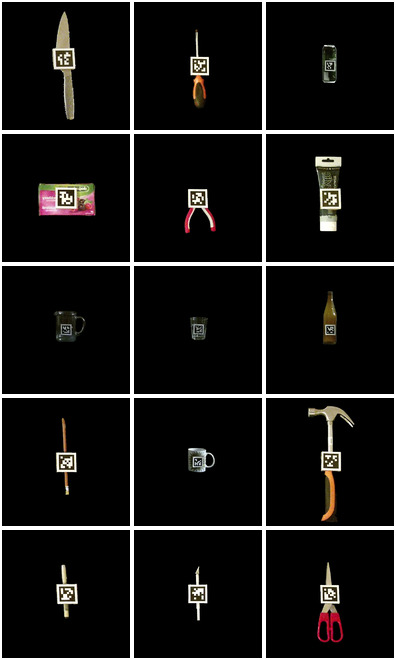
\includegraphics[width=\textwidth]{img/methods/objects.jpg}
	\caption{Ground truth images of the objects used with an AprilTag fastened to them}
	\label{fig:objects_montage}
\end{figure}

\begin{figure}
	\centering
	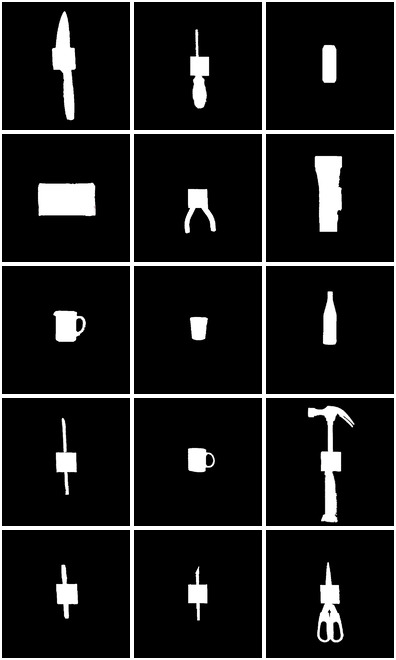
\includegraphics[width=\textwidth]{img/methods/masks.jpg}
	\caption{Binary mask of each object}
	\label{fig:masks_montage}
\end{figure}

One of our biggest challenges with the project is to actually detect the object in each frame. This is a very non-trivial task and there is much research around methods for object detection. To help us with this part of the project and make esure that the data we extract is accurate, we will use AprilTags. They can easily identify the four corners of the tags in a frame and by this way locate the object. Using the OpenCV library and their \texttt{findHomography} function, we can compute the homography matrix that transforms the four corners of the tag in the reference image to the corners of the tag found in the frame. A homography matrix \(H\) is a 3x3 matrix with a total of nine values which creates quite a few features if we would try and cluster on it. Also it contains data on how to translate the object in three-dimensional space, which in our case is irrelevant as we are only interested in a way of defining the orientation of the object and are only working with two-dimensional data.

Alternatively we can calculate a rotation of the object and through an angle represent its orientation with instead only one feature. As we are only working with two-dimensional data we will only interest ourselves for the rotation on the z-axis. From the homography we can calculate a rotation matrix from which we can later derive the searched angle. Using the Python code presented in \ref{lst:rotation_matrix} based on the OpenCV library, we compute a 3x3 rotation matrix \(R\). Using the rotation matrix we can compute the angle \(\theta_R\) as \(\theta_R = \arctan(R_{1,0} / R_{0,0})\). In this case the rotation will be around the center of the tag because it is from which we calculated the homography matrix.

The previous homography matrix can though still be used to transform the binary mask of the object, and then be applied on the frame as to mask out only the object. From this we can afterwards retrieve a grasp region of the object.

\begin{lstlisting}[
	language=Python,
	frame=single,
	label={lst:rotation_matrix},
	caption={Python code to calculate rotation matrix from homography matrix using OpenCV and numpy libraries (taken from \parencite{OpenCVHomographyDemo})},
	float,
	floatplacement=H,
	]
norm = np.sqrt(np.sum(H[:,0] ** 2))
H /= norm
c1 = H[:, 0]
c2 = H[:, 1]
c3 = np.cross(c1, c2)

R = np.zeros((3, 3), dtype=np.float64)
for i in range(3):
	R[i, :] = [c1[i], c2[i], c3[i]]
w, u, t = cv2.SVDecomp(R)
return np.dot(u, t)
\end{lstlisting}

\subsubsection{Grasp features}

Skin color is a quick way of segmentating and finding grasp region as the color of skin is quite different from the colors of the objects, but the method is not too robust in covering many different people as the color can vary quite a lot from person to person. The setting for skin color had to therefore be tweaked manually depending on the participant. By using the homography matrix and the binary image, we have been able to mask out the object from the scene. This image of the found object is later segmentated by skin color. A contour expressed as a rotated rectangle is then calculated around the largest segmentated region found, which represents our grasping region.

A rotated rectangle is composed of three different parameters: width, height and angle. Another possible feature we can extract is the ratio between area of grasp region and area of object. Using the binary image of the object we can compute its area \(A_{object}\) with the help of OpenCV by using \texttt{findContours} and \texttt{contourArea}. The area of the rotated angle is simply \(A_{grasp} = width \times height\) and the ratio between them becomes \(A_{ratio} = \frac{A_{grasp}}{A_{object}} \).

The last features that we can extract are: the distance \(\Delta\) as the L2 norm between centers of the grasp region \(O_{grasp}\) and center of mass of the object \(O_{object}\), and the direction between these centers. The center of mass can be computed using the image's moments of the binary image. Moments are retrieved with the help of the \texttt{moments} function, part of the OpenCV library, then the following formula gives us the center:

\[
	O_{object} = \frac{M_y}{M}, \frac{M_x}{M}
\]

We can then extract the distance between center of mass of the object and the center of the grasping region as a feature. It also enables us to create a unit vector from the center of mass of the object towards the grasping region. A vector in two dimensions would be expressed with two values, but we can summarize this in one value by instead calculating the angle on the z-axis by using \(\tan(\theta_G) = \sqrt{x^2 + y^2}\).

To summarize we can extract the following features:
\begin{itemize}
	\item Rotation of object in z-axis, extracted from the homography matrix of the AprilTag.
	\item Distance between center of mass of the object and the center of the grasping region.
	\item Angle between the two mentioned centers.
	\item Ratio of area of the grasping region by the area of object.
	\item Width of grasp region.
	\item Height of grasp region.
	\item Angle of grasp region.
	\item Center of grasp region.
	\item Center of mass of the object.
\end{itemize}

With these features we define for a robot how to grasp an object and present it to a human for a handover.  This list of features is however quite large and represents a very high-dimensional set of data. High-dimensionality can become quite problematic as the values might not vary with the same amount in all dimensions. We will later look at ways on reducing the number of dimensions. More on the role of the features for clustering will be presented in the results and discussion section.

\subsubsection{Filtering of unwanted frames}

One recording session consists of one pair of volunteers during which the one giving has handed over all objects in the set to the receiver. In this project we only interest ourselves for the features that define how an object is to be presented to the one receiving it, i.e. the actual moment in the end of the handover motion when the giver holds out the object ready for the receiver to take it. At all times of this session the application is continuously recording, creating a large number of frames that are of no interest such as when the participant handing over the objects is fetching the next one or the person receiving is putting one of them away. Some preprocessing of the frames is therefore required to find the frames of interest.

A first step is to create a Region of Interest (ROI) in which we will concentrate on searching for objects. This will not only help filter out the vast amount of frames that are not of interest, it will also help with performance as opposed to if we were searching the entire frame. Our ROI is arbitrarely set to the middle of the frame where the person handing over the object would finish the movement, and set to be large enough to detect the tag and see the entire object. When a tag is detected within the ROI we flag this frame to be a handover moment before extracting the features. This is unfortunately not enough because we might be flagging frames where the receiver is holding the object after taking it, or maybe both are holding it but the system detects the receiver's hand as the largest grasping region. Figures \ref{fig:handover_bottle} and \ref{fig:handover_hammer} demonstrate frames that the system detected as handovers with the objects masked out and the grasping region identified. The methods explained above might also be incorrect as the grasping region was incorrectly detected. Manual filtering was later applied to images that were flagged as handover moments and to make sure they were correct ones and that the data extracted was correct. Figure \ref{fig:handover_incorr} illustrates a situation that needs to be manually filtered out when the system percieves to have identified a handover situation but the grasping region identified is that of the receiver's.

\begin{figure}
	\centering
	\begin{subfigure}[t]{\textwidth}
		\centering
		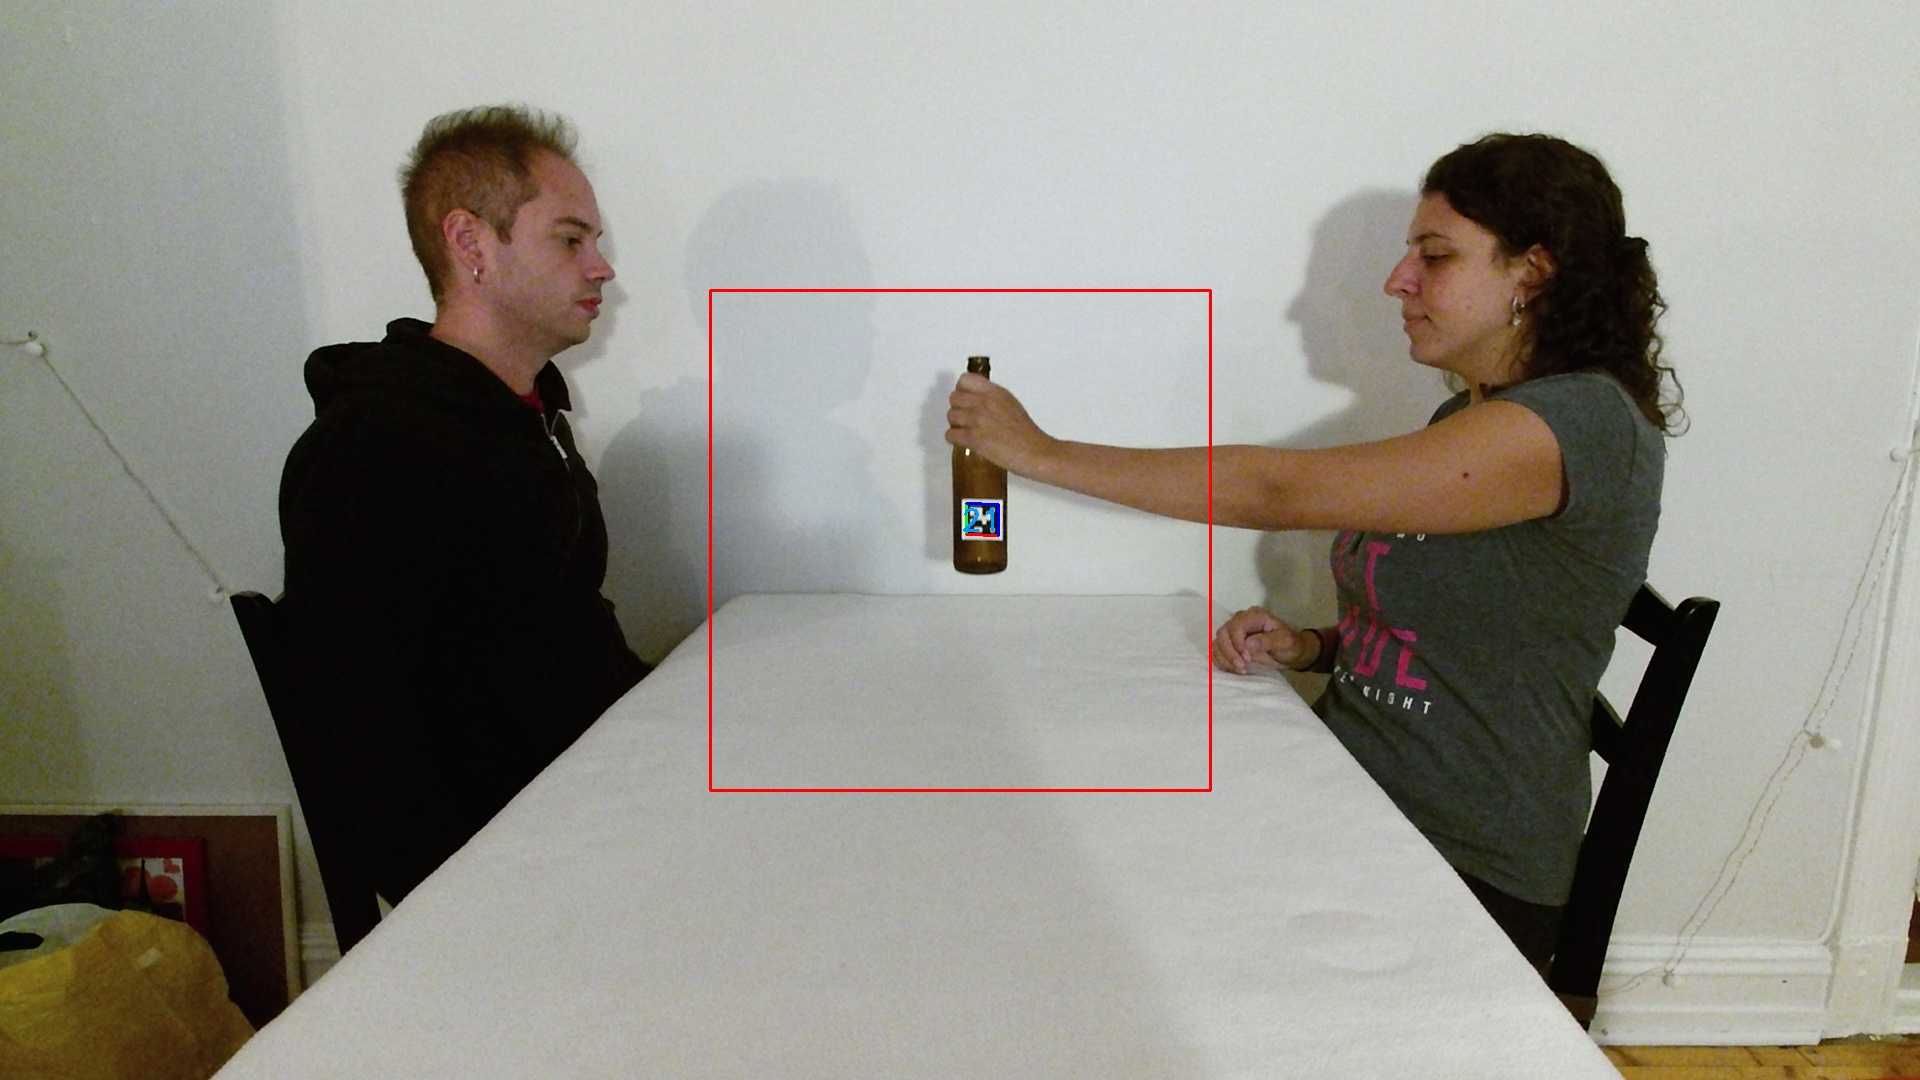
\includegraphics[width=\textwidth]{img/methods/handovers/bottle_frame.jpg}
		\caption{Handover of bottle.}
		\label{fig:demo_handover_bottle}
	\end{subfigure}
	\par\bigskip
	\begin{subfigure}[t]{0.5\textwidth}
		\centering
		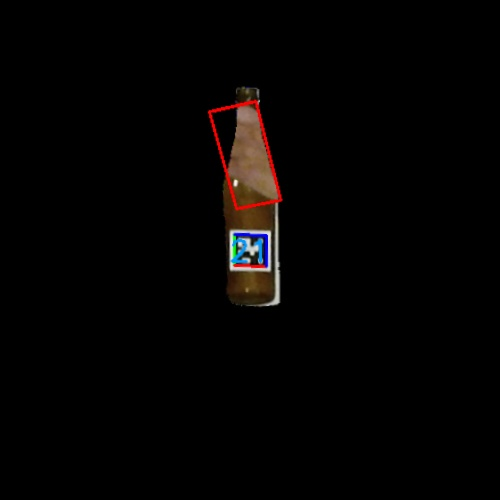
\includegraphics[width=\textwidth]{img/methods/handovers/bottle_masked.jpg}
		\caption{Bottle masked out and grasp region identified.}
		\label{fig:handover_bottle_masked}
	\end{subfigure}
	\caption{Handover demonstation of a bottle with the grasp region detected after being masked out. The giver was instructed to pretend like the bottle was full of liquids to make sure they held it upright.}
	\label{fig:handover_bottle}
\end{figure}

\begin{figure}
	\centering
	\begin{subfigure}[b]{\textwidth}
		\centering
		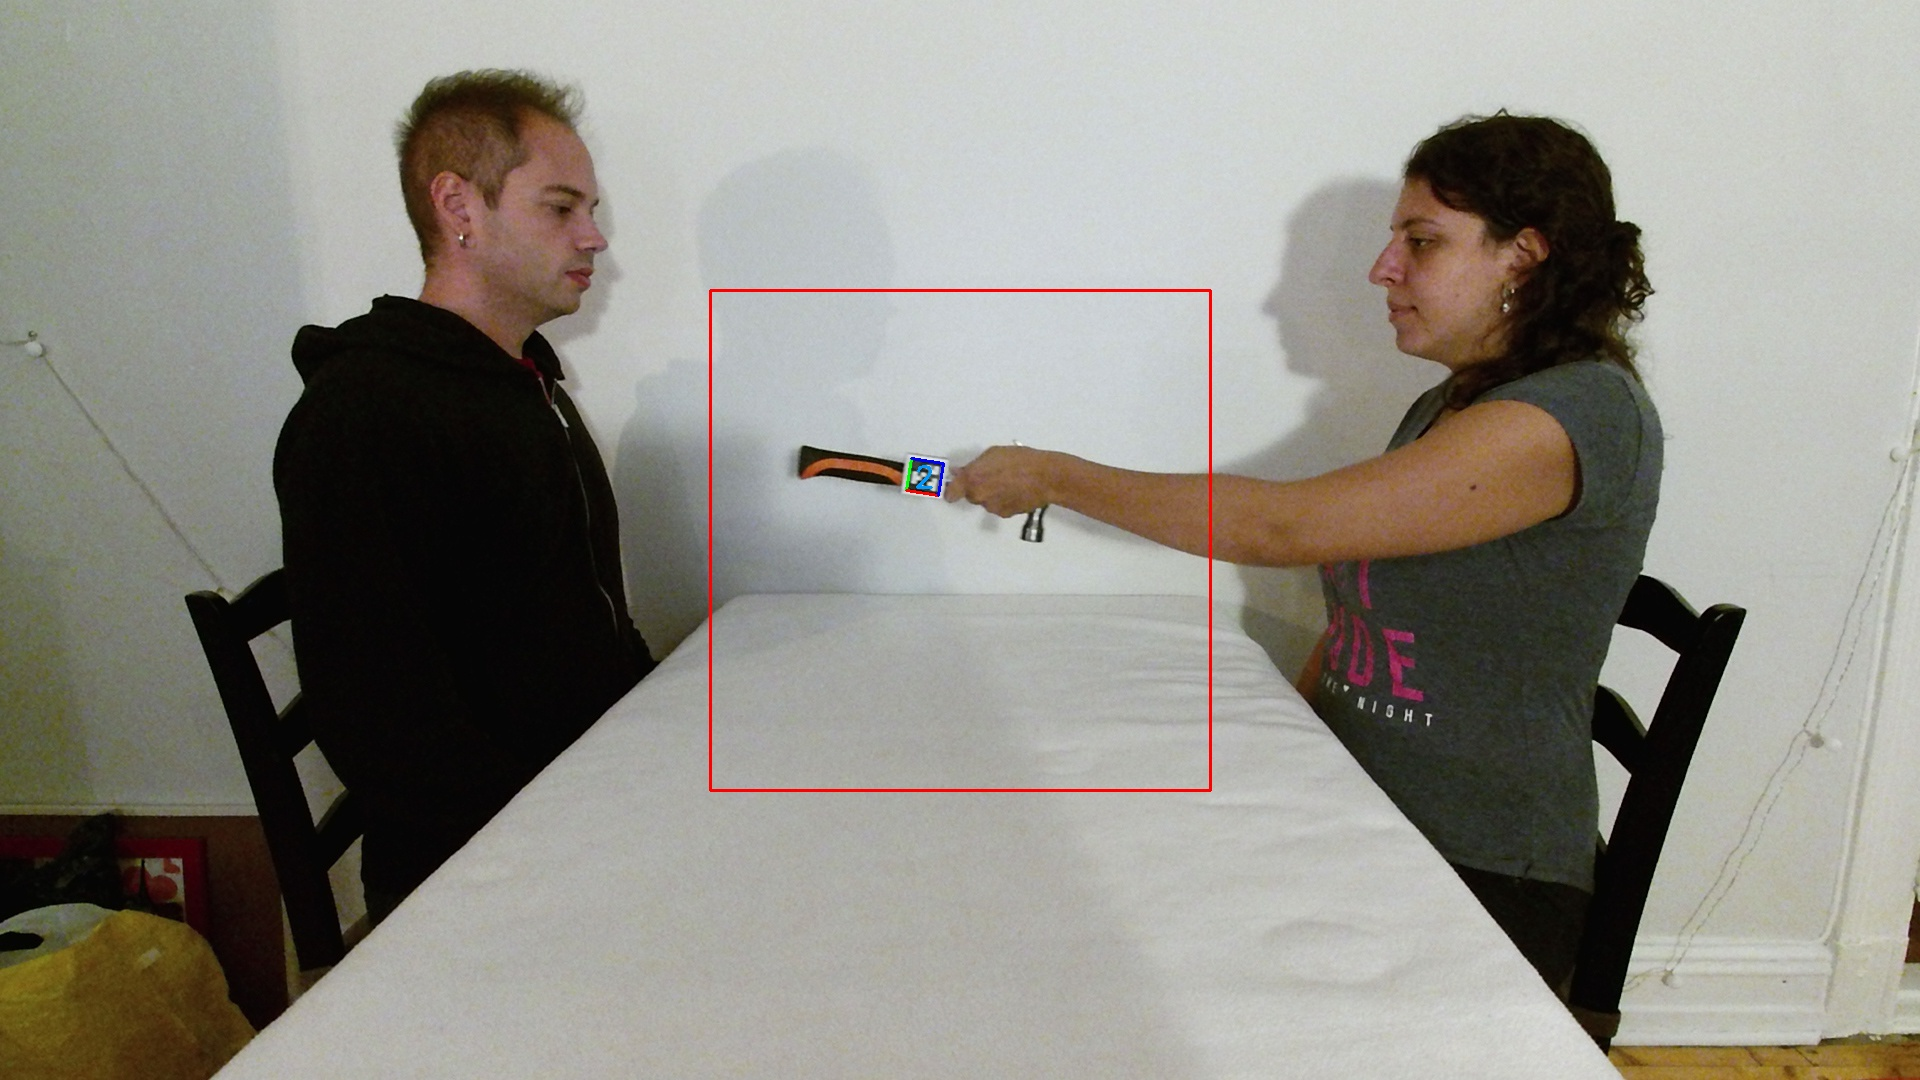
\includegraphics[width=\textwidth]{img/methods/handovers/hammer_frame.jpg}
		\caption{Handover of hammer}
		\label{fig:demo_handover_hammer}
	\end{subfigure}
	\par\bigskip
	\begin{subfigure}[b]{0.5\textwidth}
		\centering
		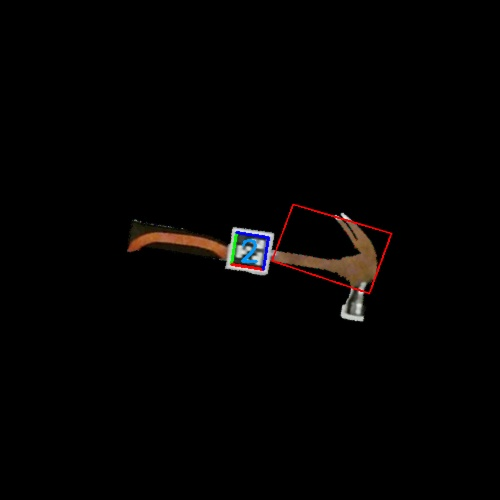
\includegraphics[width=\textwidth]{img/methods/handovers/hammer_masked.jpg}
		\caption{Hammer masked out and grasp region identified.}
		\label{fig:handover_hammer_masked}
	\end{subfigure}
	\caption{Handover demonstration of a hammer with the grasp region detected after being masked out. The giver was instructed to give it handle first, holding the head so the receiver is able to use it straight away.}
	\label{fig:handover_hammer}
\end{figure}

\begin{figure}
	\centering
	\begin{subfigure}[b]{\textwidth}
		\centering
		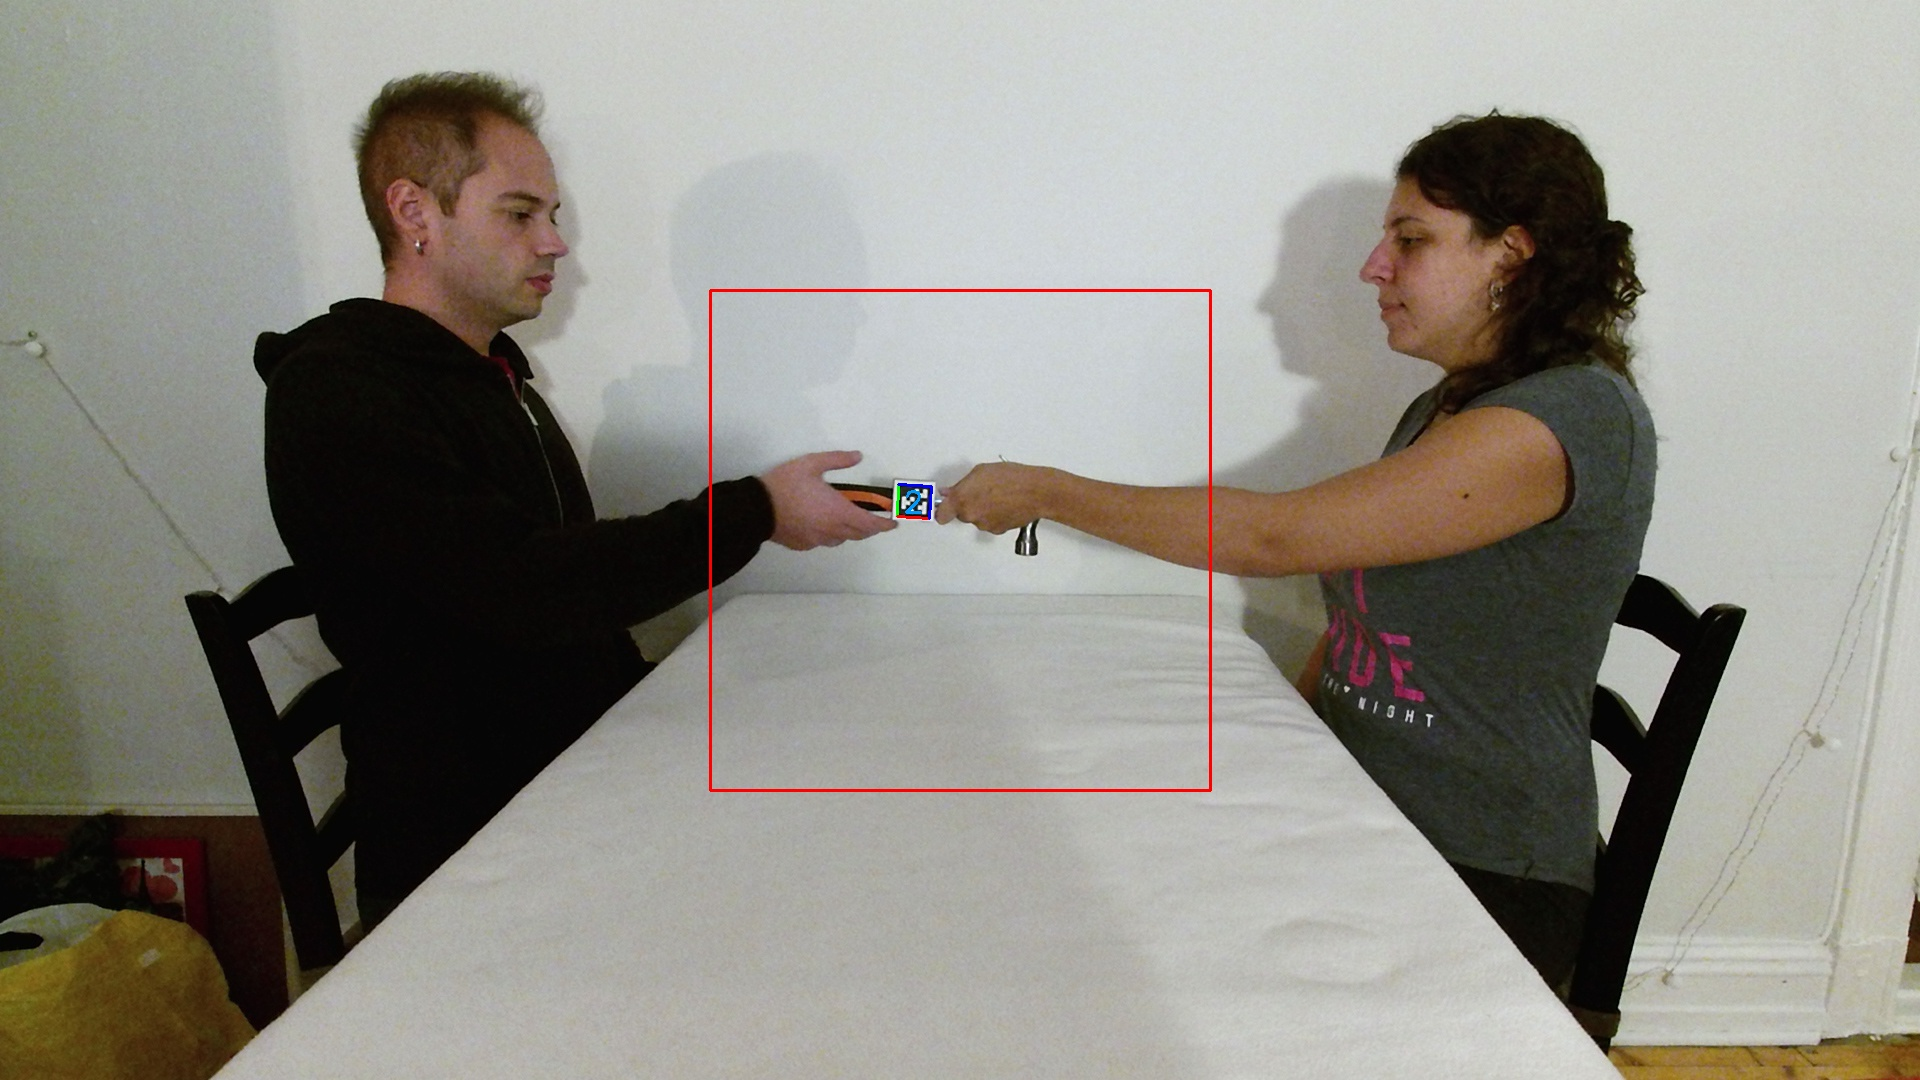
\includegraphics[width=\textwidth]{img/methods/handovers/incorr_frame.jpg}
		\caption{Handover of the hammer after the receiver takes the object.}
		\label{fig:demo_handover_incorr}
	\end{subfigure}
	\par\bigskip
	\begin{subfigure}[b]{0.5\textwidth}
		\centering
		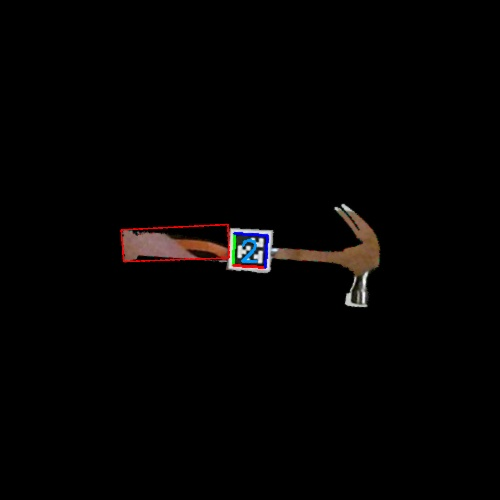
\includegraphics[width=\textwidth]{img/methods/handovers/incorr_mask.jpg}
		\caption{Hammer with the grasp region of the receiver identified.}
		\label{fig:handover_incorr_masked}
	\end{subfigure}
	\caption{Example of frame with false positive. The object is detected within the region of interest but the identified grasping region is not that of the giver, but the receiver's.}
	\label{fig:handover_incorr}
\end{figure}


\subsection{Clustering by handover features}

After observing a number of handovers betweens humans, a first step is to try and categorise these handovers into different classes that can be applied for the objects. As we do not have any labels, or even unsure how many different categories of handovers we have recorded, we will attempt at clustering using an unsupervised learning algorithm by the features that we have extracted from the recorded material.

\subsubsection{K-Means} % TODO write this section better

For the purpose of categorizing the handover samples we will be using the \emph{k-means} algorithm. K-means is an algorithm that attempts to classify a number of observations into \emph{k} number of clusters. The algorithm starts by creating \emph{k} number of centroids for each cluster and assigning our samples to the centroid within shortest distance. The algorithm iteratively then updates the centroids to become the mean of the samples assigned to it, and then re-assigns all samples depending on the new centroids. This is repeated either a fixed number of times or until the algorithm converges minimizing the sum of squares within the clusters.

\subsubsection{Principle component analysis (PCA)} % TODO write this section better

A challenge that presents itself using clustering algorithms is choosing what features are to be used for the purpose and how many clusters should we create. We will be using \emph{Principle component analysis} (PCA) to evaluate which features that are to be used to define each cluster. Ideally we use the smallest number of features possible, but also the ones that create the most distinct clusters, which PCA will help us with. Before using techniques such as PCA to minimize the amount of features that are needed to cluster we will try to define what features matter in a handover and deduct them from the data we have, as well as trying to redefine some features in a more compressed matter.



%
% Prediction of handover class
%


\section{Prediction of handover class}

As mentioned our aim in the end is to have a robot be able to predict a handover setting given an image of an object. In our case we will have it predict a class of handovers which are the result of the previous clustering. The system needs in this case to be able to relate visual features that come through imagery, to the class, also in a sufficiently abstract way that it can accurately predict the class for an unencountered object during training.

\subsection{Convolutional Neural Networks}

We hypothesize in this case that there is a number of features that can be retrieved visually from the objects, that define which class of handovers it belongs to. Even though we could try and preprocess all sets of objects and re-define them as a set of features, such as decomposing them into geometrical shapes, choosing which features it should be and how to retrieve them would be a challenging task, especially before knowing the results of the clustering. In \ref{sec:machine_learned_systems} we mentioned convolutional neural networks and works such as \parencite{Lee2009}, \parencite{Turaga2010} where the layers through training are able to hierarchically extract features in the images to later perform precise visual tasks. This ability of CNNs corresponds well with our goal to have the machine learn atonomously without human preprocessing or labeling. Through training on a dataset of images, our hope is that the machine will be able to draw relations between visual features extracted from the images with a certain class of handovers.

\subsection{AlexNet network}

For the task of predicting handover class from an image we will be training a convolutional neural network. The most challenging part with all artificial neural networks is to define their architecture. Changes to the number of layers and their sizes can play a significant role on the outcome of the results. Within object classification there have been a number of architectures proposed that have achieved good results, one of these is the \texttt{AlexNet} network which was mentioned in \ref{sec:machine_learned_systems}, and we will use as basis for our own network.

The AlexNet was designed for the ImageNet object classification problem in 2010, trained over 1,2 million images to output 1000 different classes. As a reminder, figure \ref{fig:alexnet_orig} shows the network architecture used by the AlexNet. It includes in total eight layers, all of which use ReLU non-linearity as activation function:

\begin{description}

	\item[Five convolutional layers] The first convolutional layer filters the \(224 \times 224 \times 3\) input image with 96 kernels of size \(11 \times 11 \times 3\) with a stride of 4 pixels. The second convolutional layer takes as input the (response-normalized and pooled) output of the first convolutional layer and filters it with 256 kernels of size \(5 \times 5 \times 48\). The third, fourth, and fifth convolutional layers are connected to one another without any intervening pooling or normalization layers. The third convolutional layer has 384 kernels of size \(3 \times 3 \times 256\) connected to the (normalized, pooled) outputs of the second convolutional layer. The fourth convolutional layer has 384 kernels of size \(3 \times 3 \times 192\) , and the fifth convolutional layer has 256 kernels of size \(3 \times 3 \times 192\).

	\item[Three fully connected layers] with 4096 neurons each, where the last one is fed to a 1000-way softmax output.

\end{description}

In total the network consists of 60 million parameters and 650 000 neurons. At the time, the designers of the network were under the restriction of the performance of GPUs, hence the parallell system. Seeing how our classification problem is of significantly smaller scale its size will do without problem, note however that we will re-design it so it runs sequentially on one GPU. The only other modification we will attempt will be by adding a new fully connected layer at the end with size depending on the results from the prior clustering. Figure \ref{fig:method_cnn_arch} shows our network architecture. As a side note: since the AlexNet network was designed, several other successful network architectures have been proposed, some that even outperform AlexNet. Such as \texttt{VGG-16} by \textcite{Arge2015} and \texttt{Inception} by \textcite{Szegedy2014}. These networks are however larger and deeper which would in theory require more processing time and as well as more data to train, both which are of limited supply. The AlexNet therefore makes a good compromise and should still be well suited for our smaller problem.

\begin{figure}
	\centering
	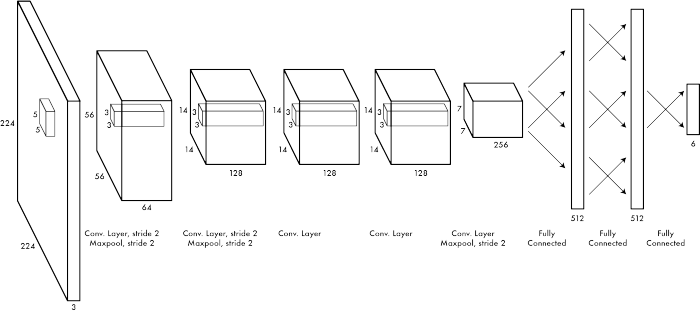
\includegraphics[width=\textwidth]{img/related-work/cnn-architecture.png}
	\caption{\textcolor{red}{insert correct graph}}
	\label{fig:method_cnn_arch}
\end{figure}

\subsection{Training and testing}

We want the machine to learn from the handovers between humans that it has observed. We will therefore only use as our dataset the objects that were used for recording handovers. Despite their potential for performing very well, one issue with ANNs (especially very deep ones) is that they often require a lot of data to do so. The amount of data we are able to gather by taking images of the objects is unfortunately not enough for a network as large as the AlexNet network which was designed for over a million images. Fortunately for us there are pre-trained weights to be found that we can work upon and increase our chances of success. At \parencite{AlexNetImplWeights} we can find a set of pre-trained weights to use and also we can find a good base for our own implementation of the architecture using the Python library \texttt{tensorflow}.  Next step is to finetune the pre-trained weights to better fit our own data and fit it to our desired output.

Color images contain three channels of color (RGB) to define their texture. We theorize that it is not only the texture that defines the visual features of a handover class but also the shape of the object. Three channels of color can therefore feel redundant if the color is not the only thing that defines what the objects have in common. It can also create distinctions between the objects that are unnecessary and maybe confusing for the network to learn as it will make it harder to learn relations between them. Depth data gives a good 2,5-dimensional representation of the shape of the object, which can also be visualized by converting it to a grayscale image. This can be seen as one channel of color. As input data we will be taking inspiration from \parencite{Redmon2014} and perform the same alterations to our own dataset by replacing the blue color channel with the depth image. Figure \ref{fig:rgbd} shows an example of the hammer with its RGB image to the left, depth image in the middle and to the right the color image with the blue channel replaced for the depth data. Using the Kinect v2 camera, both color and depth images were taken of all objects from several different angles in different positions. Data augmentation was later performed on the resulting images to enlargen the dataset by using flipping, random cropping and random rotations of the images.

There are issues like black triangles in the corners or along the edges after rotating and/or cropping. These images are unwanted as the network might identify these regions with the objects. Therefore all the images created through data augmentation will be gone through manually as to make sure they are all suitable for training by the network. After we are done selecting images for our dataset we are not guaranteed that it is balanced between the objects or the classes. To prevent any overfitting we will also make sure that we balance the dataset evenly over all objects and classes.

\begin{figure}
	\centering
	\begin{subfigure}[b]{0.3\textwidth}
		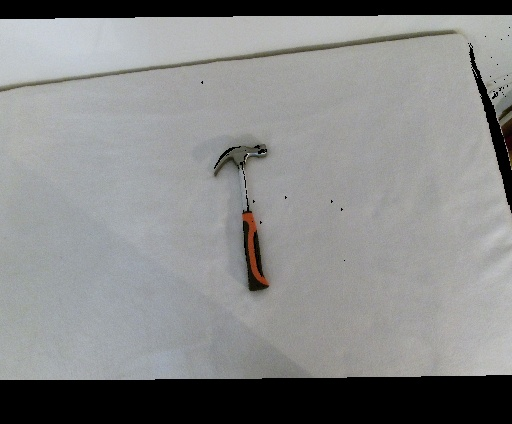
\includegraphics[width=\textwidth]{img/methods/rgbd/rgb.jpg}
	\end{subfigure}
	\begin{subfigure}[b]{0.3\textwidth}
		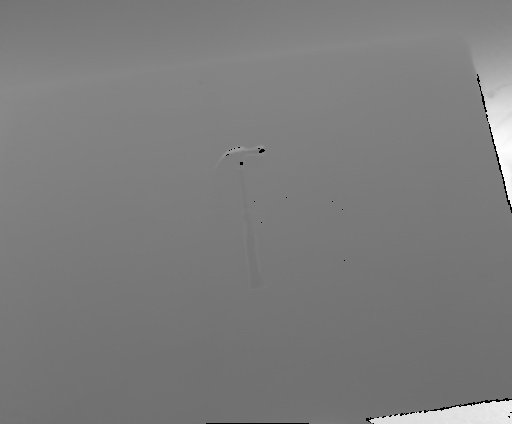
\includegraphics[width=\textwidth]{img/methods/rgbd/depth.jpg}
	\end{subfigure}
	\begin{subfigure}[b]{0.3\textwidth}
		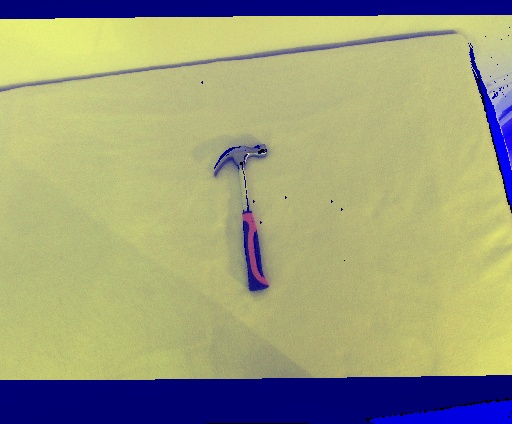
\includegraphics[width=\textwidth]{img/methods/rgbd/rgbd.jpg}
	\end{subfigure}
	\caption{RGB-, depth- and RGB-image with blue channel replaced by the depth data for the hammer.}
	\label{fig:rgbd}
\end{figure}

Training and validation will be performed on a larger subset of the images to see how well the system is able to recognize and predict a class for objects it has been trained for. While a smaller subset will be used later for testing to see how well the system performs on foreign objects that it has never seen before. The sizes of these subsets will be varied as to see how many objects are required for training to perform well on new objects.
